\documentclass[11pt]{article} % 72pt = 1 inch
\textwidth=35pc         % a bit wider than the default, 1 pica = 1/6 inch
\hoffset=-2pc
\textheight=54pc        % a bit taller than the default
\topmargin=-3pc         % moves text up to center
\linespread{1.5}        % gives about one-and-one-half line spacing
\usepackage{graphicx}
\graphicspath{{images/}}


\begin{document}

\begin{center}
\large
\bf
ANLY-550 Homework 4 \\[1pc]
\rm
\normalsize
Yi Li, Apr. 19 \\[1.5pc]  
\end{center}


\normalsize
\noindent
1. 
$$
\begin{array}{c|c|c|c|c|c|c|}
H & x=1 & x=2  \\ \hline
h_1(x) = (x-3/2)^2 + 3/4 & 1 & 1 \\ \hline
h_2(x) = x  & 1 & 2 \\ \hline
\end{array}
$$ 

We see that $Pr_{h \leftarrow H}[h(1)=1 \cap h(2)=2] = 1/2 \neq 1/4$, so $H$ is not pairwise independent.
We see that $h_1(1) = h_1(2), h_1(1) \neq h_2(2), h_2(1) = h_1(2), h_2(1) \neq h_2(2)$, so $Pr_{h \leftarrow H}[h(1)=h(2)] = 2/4 = 1/2$. Thus, $H$ is universal.
\\

\noindent
2. We can consider all balls as two categories: blue balls and non-blue balls. The probability to see a blue ball with $n$ random draws is $P_{blue} = 1 - x^n$, where $x$ is the percentage of non-blue balls of all balls. 
The goal is to calculate the smallest $n$ such that $P_{blue} \geq 2/3$.
We know that there are at least $10\%$ blue balls, so there are no more than $90\%$ non-blue balls, which means that $x \leq 0.9$. 
In the worst case, $x=0.9$, so solve the inequality $P_{blue} = 1 - 0.9^n \geq 2/3$,
and we get $n \geq 11$. 
So one have to draw 11 balls at random from the bag to see a blue ball with probability at least 2/3. \\

\noindent
3. As on YES instances the algorithm $A$ is always correct, so repeating the algorithm $A$ on YES instances will not change the results. While on NO instances the algorithm $A$ outputs YES with probability at most $1/2$, so if one runs the algorithm $A$ again, then the probability of outputting YES on NO instances becomes at most $1/4$. Thus, if one runs the algorithm $A$ for 100 times, the probability of outputting YES on NO instances becomes at most $2^{-100}$.

As the new algorithm $B$ runs the algorithm $A$ for 100 times, so the running time of algorithm $B$ is 100 times of the running time of the algorithm $A$. In other words, the algorithm $B$ is 99 times slower than the algorithm $A$.\\


\noindent
4. We can compute the number of independent set recursively by considering two parts: (a) the number of independent sets containing the root, (b) the number of independent sets not containing the root.

\noindent
4.1. Let $a(n)$ denotes the number of independent sets with $n$ nodes.
When there is only one node, there are two independent sets: a set with one node, and an empty set, that is, $a(1) = 2$. And when there is no node, there is only one empty set, that is, $a(0) =1$.
 
When we add a new node to the line graph (assume that now there are $n$ nodes), the number of independent sets without the root is exactly $a(n-1)$. And the number of independent sets with the root is $a(n-2)$, because the independent sets can only be the sets that the root join with its grandchildren's independent sets. So, the recursion is $a(n) = a(n-1) + a(n-2)$ for all $n \geq 2$, and $a(0)=1, a(1)=2$.\\

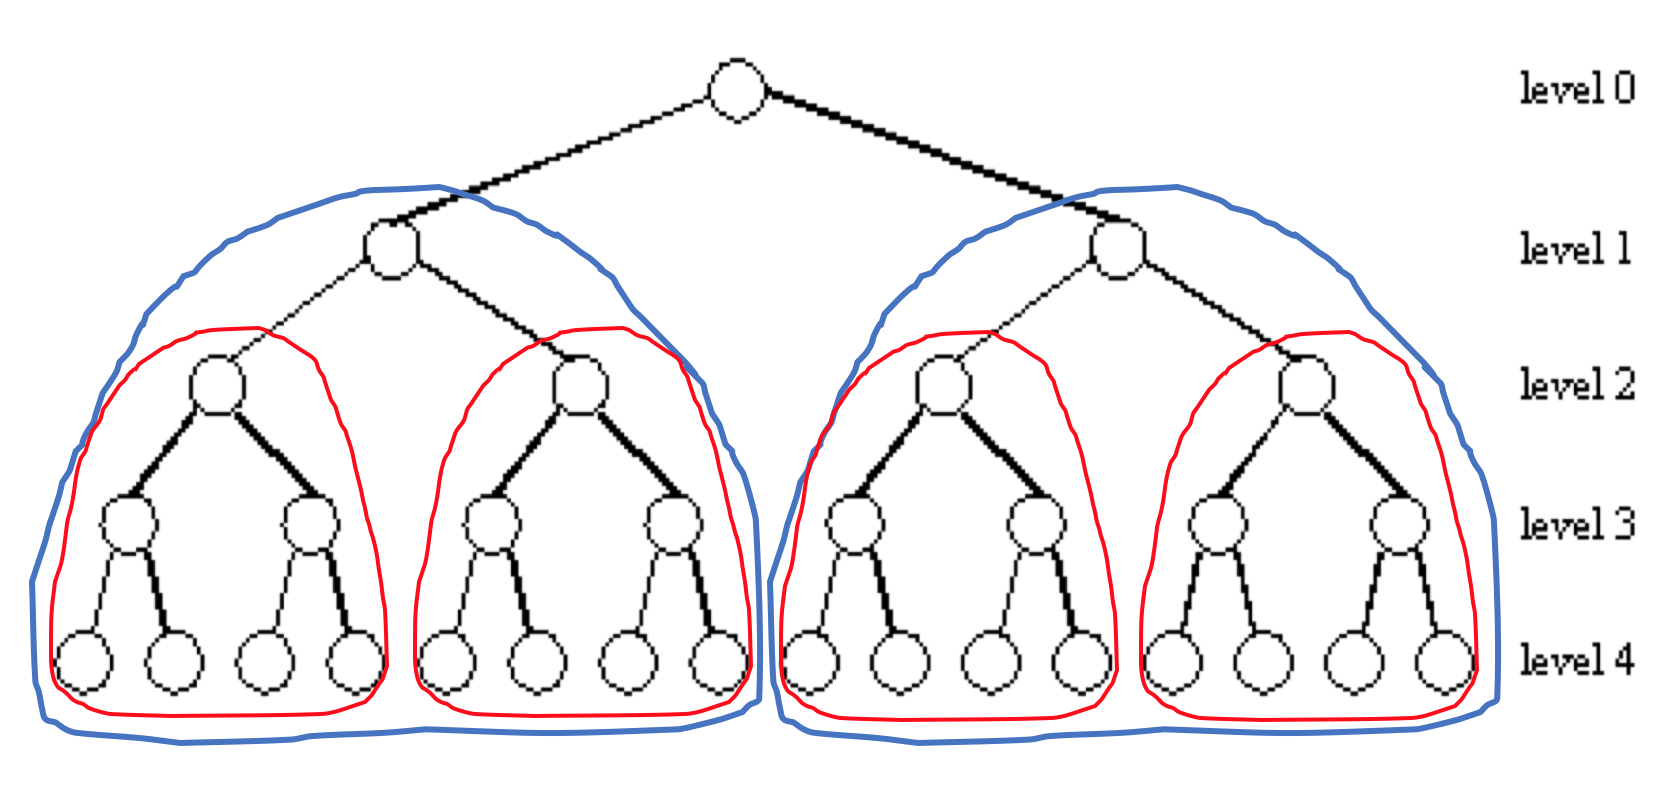
\includegraphics[scale=0.45]{figure.png}\\

\noindent
4.2. Like what we have done for the line graph, let $b(n+1)$ denotes the number of independent sets of a complete binary tree with $n$ levels. (Note: The root of a tree is at level 0.) Similarly, when there is only one node (level 0),  $b(1) = 2$. And when there is no node,  $b(0) =1$. 

When we add a new level of nodes to the complete binary tree (assume that now the tree has $n-1$ levels), the number of independent sets without the root is $b(n-1)^2$, because there are two subtrees who have  $b(n-1)$ independent sets (see two blue circles in the figure). And the number of independent sets with the root is $b(n-2)^4$, because there are four subtrees who have $b(n-2)$ independent sets (see four red circles in the figure). So, the recursion is $b(n) = b(n-1)^2 + b(n-2)^4$ for all $n \geq 2$, and $b(0)=1, b(1)=2$.

A complete binary tree with 127 nodes has 6 levels, so according to the recursion, we get $b(7) = 1.334535e+28$.\\



\noindent
5. We can reduce clique to independent set. Let $\bar{G}$ be the complement of $G$, which is the graph with the same nodes as $G$, but the edges of $\bar{G}$ are precisely those edges that are missing from $G$. Then $C$ is a clique in $G = (V,E)$ if and only if $C$ is an independent set in $\bar{G}$. 
It takes linear time to transfer $G$ to $\bar{G}$, and one can solve the decision problem that whether a graph has an independent set of size $k$ with a polynomial time algorithm. To solve the optimization problem, one can set $k = 1, 2, …, K$ until find such a $K$ that  $\bar{G}$ has an independent set of size $K$ while it does not have an independent set of size $K+1$. So the decision problem of clique has a polynomial time algorithm, and the optimization problem also has a polynomial time algorithm. \\


\noindent
6. $2Clique \in NP$: To check if $G$ has two vertex disjoint cliques of size $k$, we need to check if the two cliques $C_1, C_2$ are real cliques of size $k$ in $G$, and if $C_1, C_2$ are disjoint. As the decision version of $Clique$ is in NP-complete, the decision problem of $2Clique$ is also NP.

NP-Hardness: We can reduce $Clique$ to $2Clique$ as follows. Given an instance of $Clique[G(V,E),k]$, we create an instance of $2Clique$ by: adding a sub-graph $H^*$ which consists of a set of $k$ vertices $V^*$, and a set of edges $E^*$ such that $H^*$ is fully-connected. There will be no edges connecting the nodes in $V^*$ to the nodes in $G$. Hence we have $H(V',E')$ such that $V' = V \cup V^*$ and $E' = E \cup E^*$. 

Proof:
If $G(V,E)$ has a clique $C$ of size $k$, then by our construction, $H$ has two vertex disjoint cliques $C, H^*$ of size $k$. 
If $H$ has two vertex disjoint cliques $C, H^*$ of size $k$, then by our construction, $G$ and $H^*$ are disjoint, so $C$ must be in a subgraph of $G$, that is, $G(V,E)$ has a clique $C$ of size $k$. \\



\noindent
7.1. Considering a graph $G$ with $n$ vertices, and the optimal size for its minimum vertex cover is $x$, then the optimal size for its maximum independent set is $n-x$. Let $y$ be the size of the minimum vertex cover calculated by a polynomial 2-approximation algorithm, so $y \leq 2x$. And the size of the corresponding independent set is $n-y$.

Consider a bipartite graph $G$ with 9 nodes, whose optimal size for its minimum vertex cover is 4 and the size of the minimum vertex cover calculated by a polynomial 2-approximation algorithm is 8, so $(n-y)/(n-x) = 1/5$. Consider another bipartite graph $G$ with 11 nodes, whose optimal size for its minimum vertex cover is 5 and the size of the minimum vertex cover calculated by a polynomial 2-approximation algorithm is 10, so $(n-y)/(n-x) = 1/6$. So, one can always create some graph $G$ such that $(n-y)/(n-x)$ can be smaller than any given constants.
As $(n-y)/(n-x)$ does not have a lower boundary, a 2-approximation of the Minimum Vertex Cover does not yield an approximation algorithm for the Maximum Independent Set.



\noindent
7.2. We know that both of the Maximum Clique and the Maximum Independent Set are NP-complete, and both of them have a 1-approximation algorithm. So a 1-approximation algorithm for the Maximum Clique problem can yield a 1-approximation algorithm for Maximum Independent Set. 


\end{document}

